\section{Histograms on the Second Run~\label{sec:sodb9_r2_hist}} 
This section exhibits histograms on the second run of 
INC with its task length increasing from 1 second to 4096 seconds, via EMPv5. 
The detailed description of the base data is from Table~\ref{tab:exp_notes2}.

\begin{table}[h]
\begin{center}
\begin{tabular}{|p{2cm}|p{3cm}|p{3cm}|p{4cm}|p{3.5cm}|} \hline
Machine & Task Length (sec) & Description & Experiment Period & Relevant \linebreak Histograms\\ \hline
{\tt sodb9} &  INC1$\sim$INC64 & 1000 samples, each & 2017-03-13 $\sim$ 2017-03-14 & Figs.~\ref{fig:s9_r2_et_hist1},~\ref{fig:s9_r2_et_hist2},~\ref{fig:s9_r2_pt_hist1}, and~\ref{fig:s9_r2_pt_hist2}\\ \hline
{\tt sodb9} &  INC128$\sim$INC1024 & 300 samples, each & 2017-03-14 $\sim$ 2017-03-21 & 
Figs.~\ref{fig:s9_r2_et_hist3} and~\ref{fig:s9_r2_pt_hist3}\\ \hline
{\tt sodb10} & INC2048 & 300 samples & 2017-03-13 $\sim$ 2017-03-20 & Figs.~\ref{fig:inc2048_r2_et_hist_v5} and~\ref{fig:inc2048_r2_hist_v5}\\ \hline
{\tt sodb12} & INC4096 & 300 samples & 2017-03-02 $\sim$ 2017-03-17 & Figs.~\ref{fig:inc4096_r2_et_hist_v5} and~\ref{fig:inc4096_r2_hist_v5}\\ \hline
\end{tabular}
\end{center}
\vspace{-.2in}
\caption{Notes on experiment runs used for histograms\label{tab:exp_notes2}}
\end{table}

\pagebreak

\subsection{ET}

\begin{figure}[hp!]
	\centering
	\subfigure[ET frequency on INC1]{
		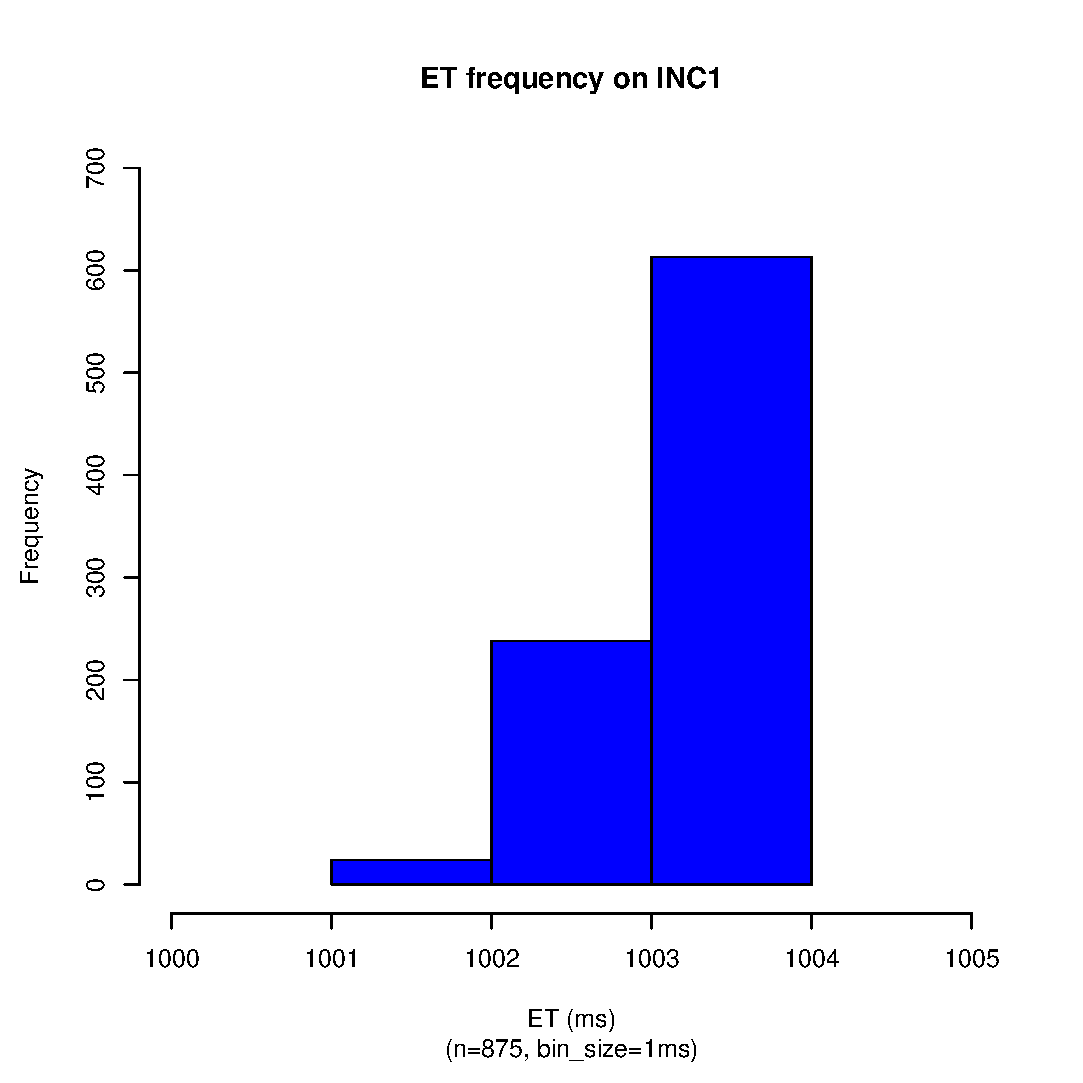
\includegraphics[scale=0.43]{repet_data1/1_sec_et_hist_v5.eps}
		\label{fig:inc1_r2_et_hist_v5}
	}
	\subfigure[ET frequency on INC2]{
		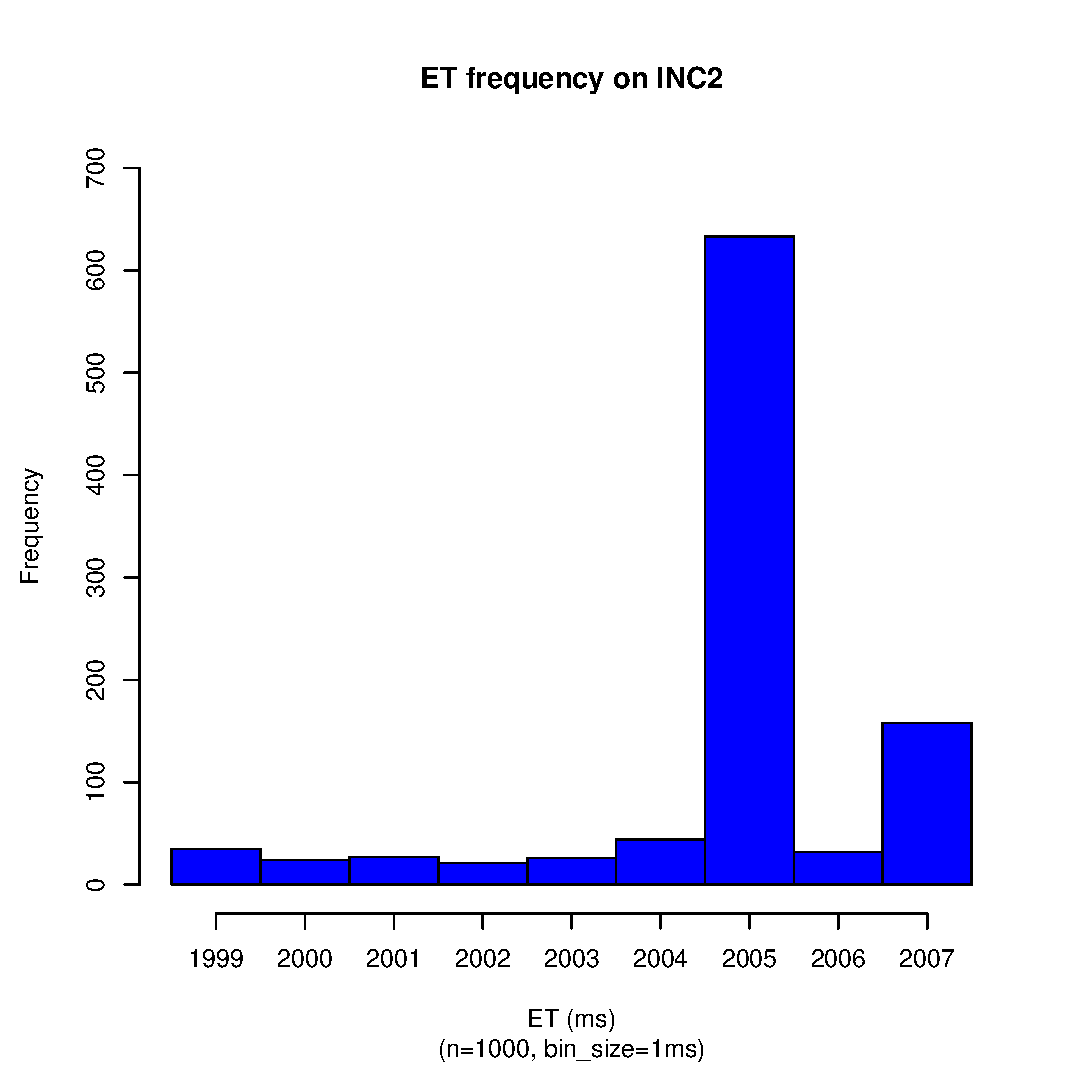
\includegraphics[scale=0.43]{repet_data2/2_sec_et_hist_v5.eps}
		\label{fig:inc2_r2_et_hist_v5}
	}
	\subfigure[ET frequency on INC4]{
		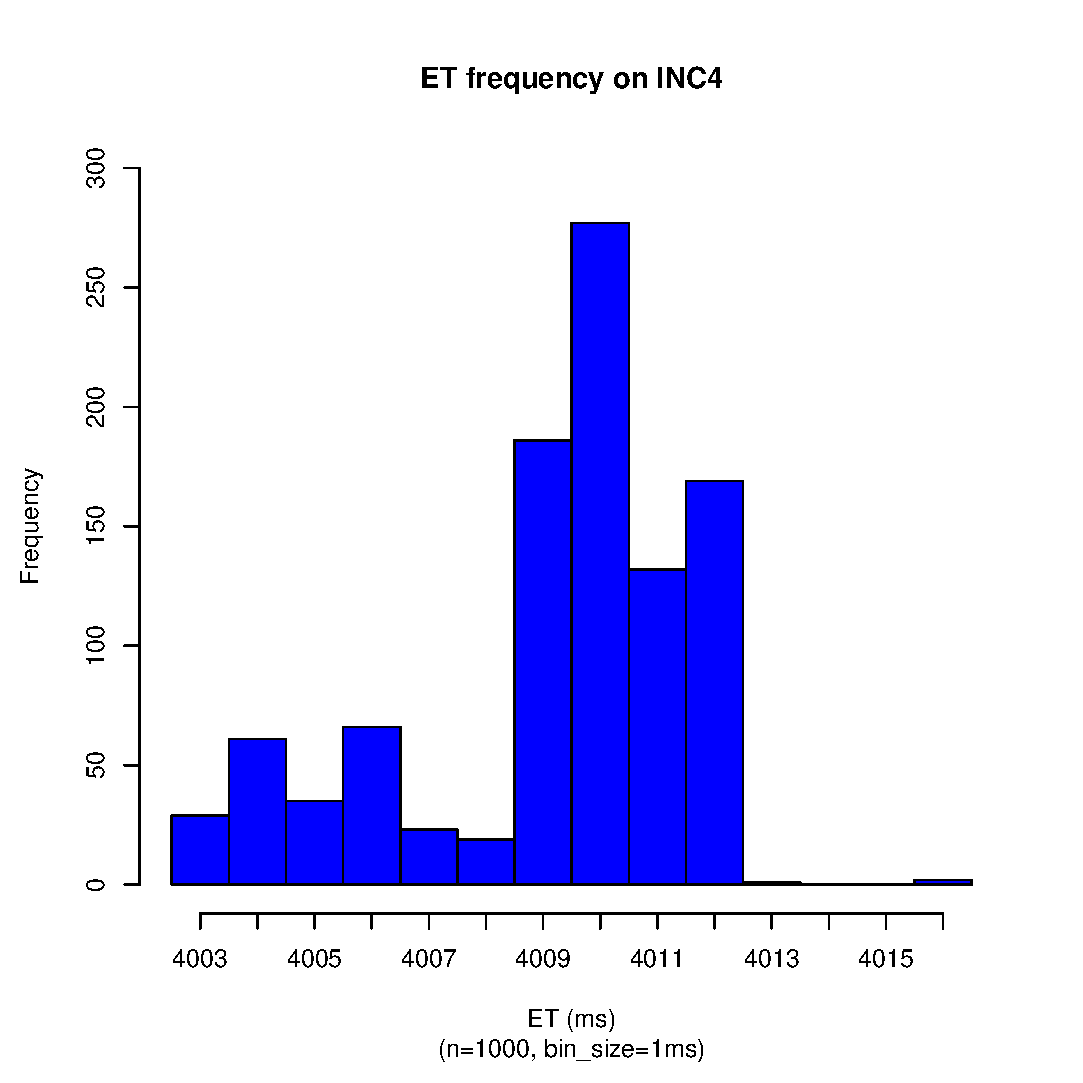
\includegraphics[scale=0.43]{repet_data2/4_sec_et_hist_v5.eps}
		\label{fig:inc4_r2_et_hist_v5}
	}
	\subfigure[ET frequency on INC8]{
		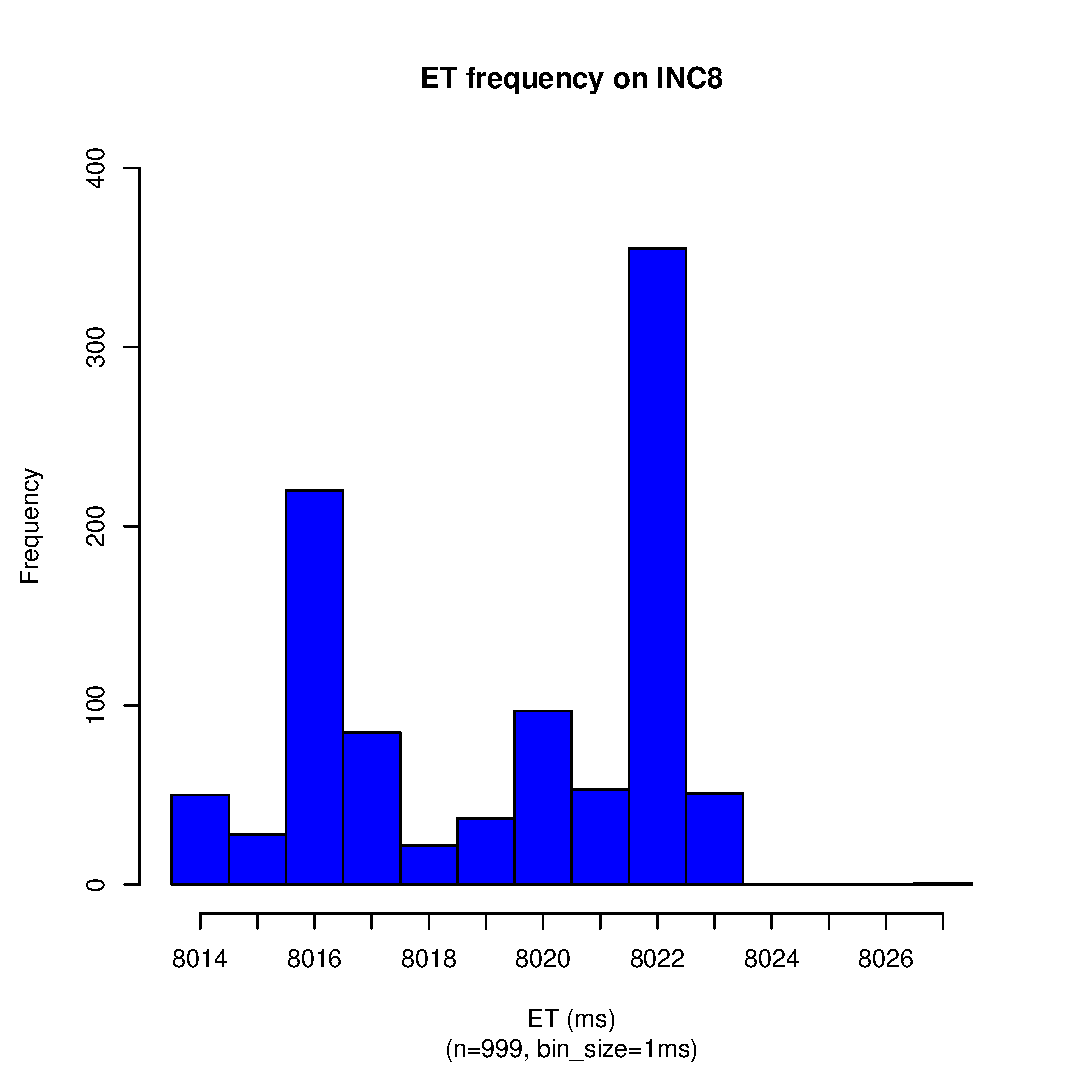
\includegraphics[scale=0.43]{repet_data2/8_sec_et_hist_v5.eps}
		\label{fig:inc8_r2_et_hist_v5}
	}
	\caption{ET Histograms of INC1 ... INC8~\label{fig:s9_r2_et_hist1}}
\end{figure}

\begin{figure}[hp!]
	\centering
	\subfigure[ET frequency on INC16]{
		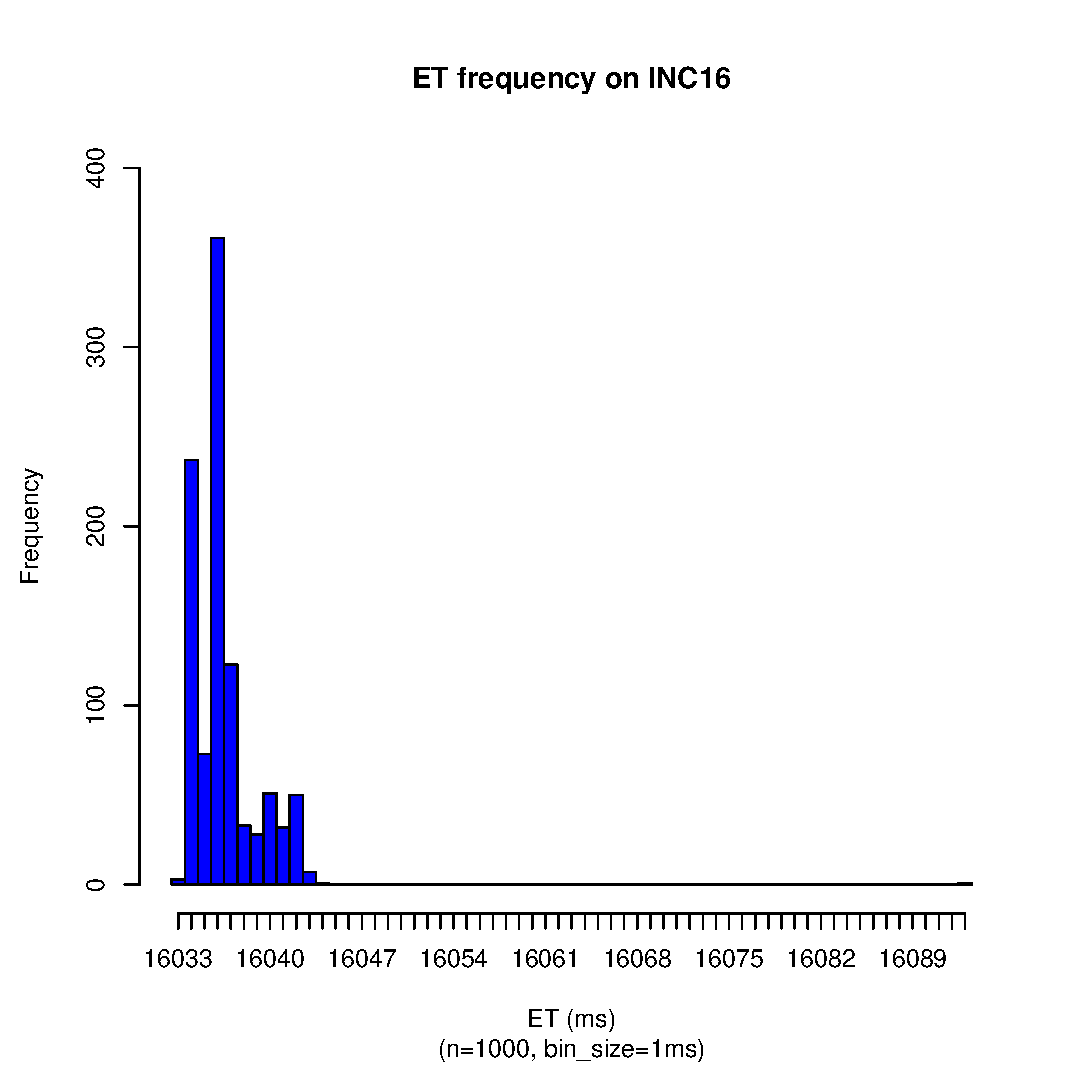
\includegraphics[scale=0.43]{repet_data2/16_sec_et_hist_v5.eps}
		\label{fig:inc16_r2_et_hist_v5}
	}
	\subfigure[ET frequency on INC32]{
		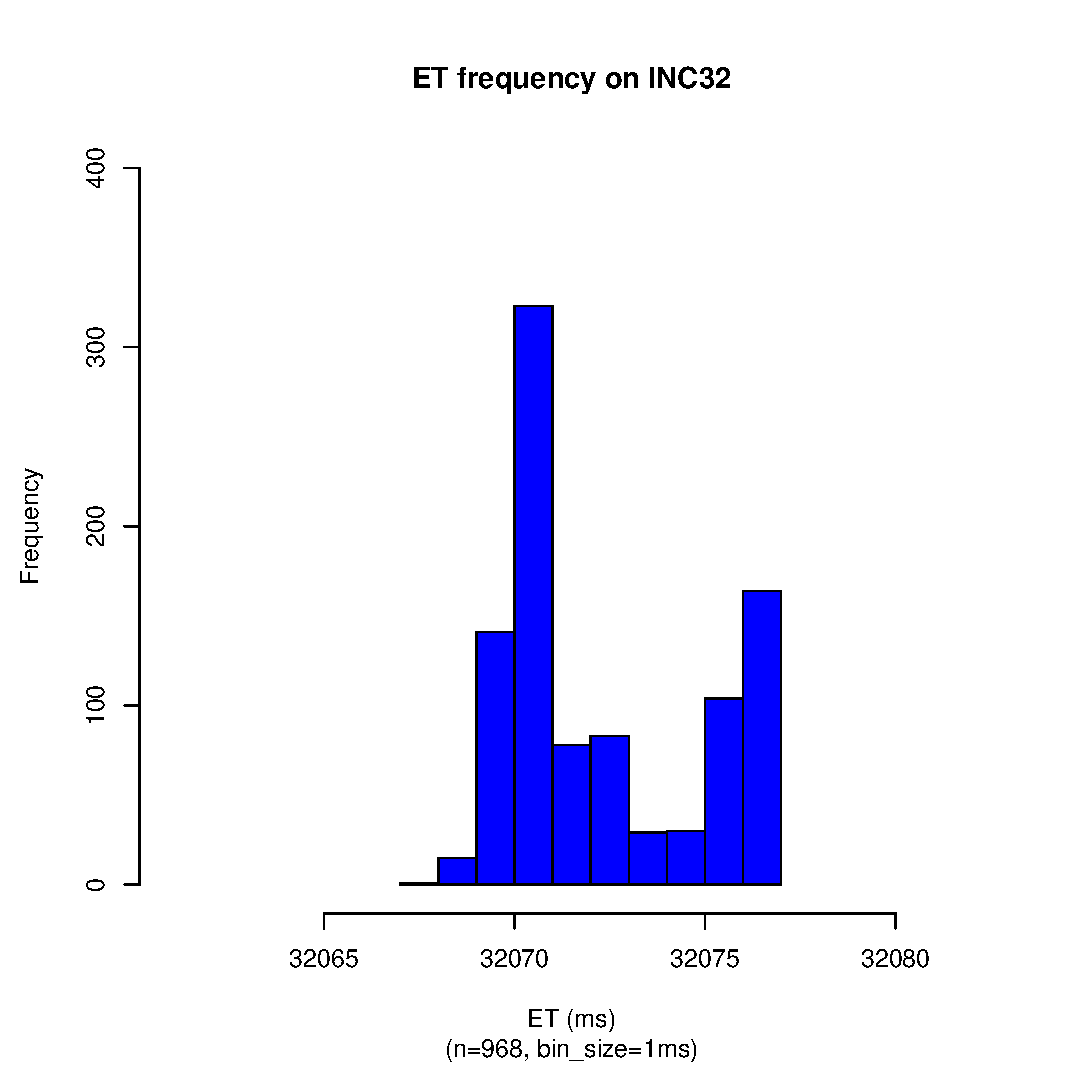
\includegraphics[scale=0.43]{repet_data2/32_sec_et_hist_v5.eps}
		\label{fig:inc32_r2_et_hist_v5}
	}
	\subfigure[ET frequency on INC64]{
		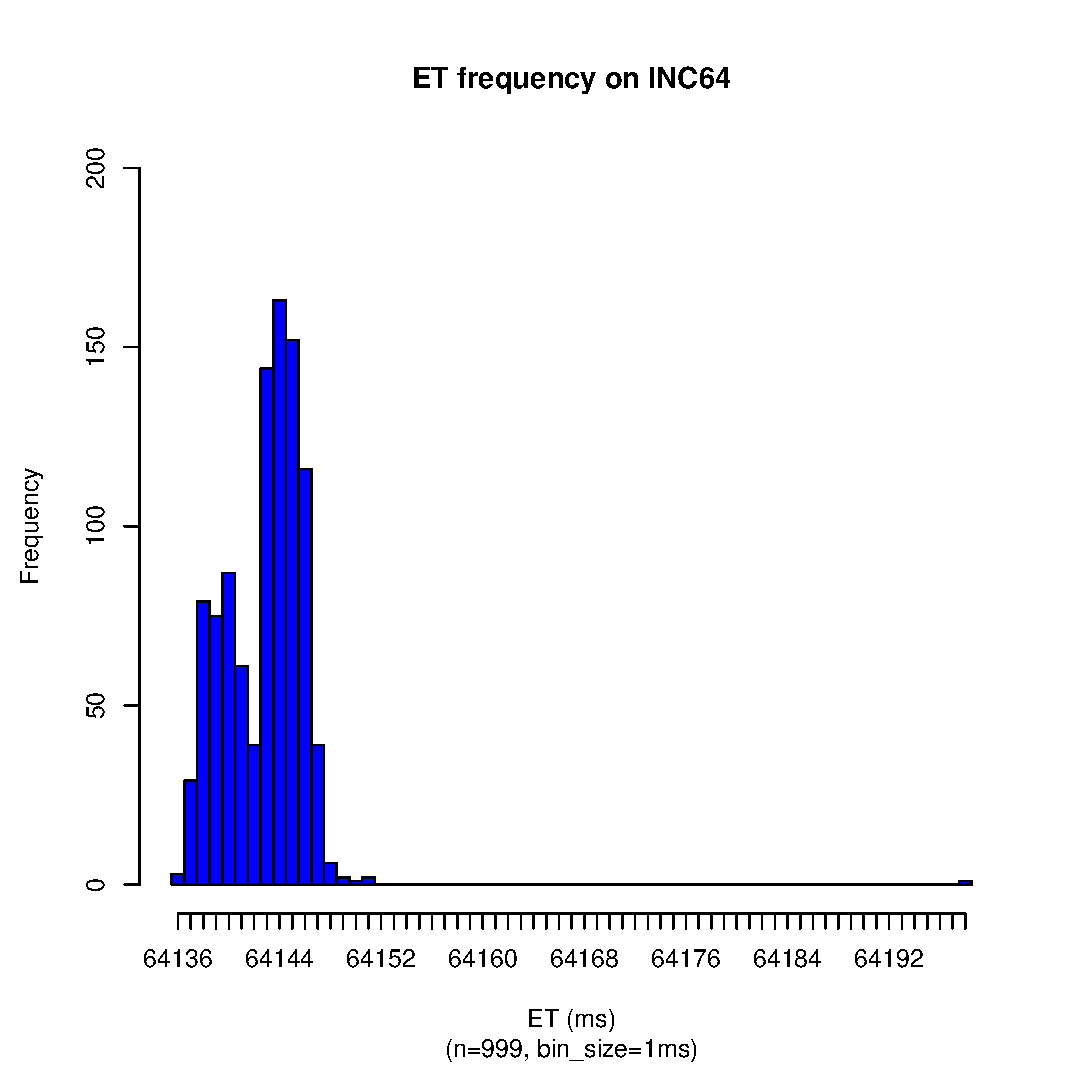
\includegraphics[scale=0.43]{repet_data2/64_sec_et_hist_v5.eps}
		\label{fig:inc64_r2_et_hist_v5}
	}
	\caption{ET Histograms of INC16 ... INC64~\label{fig:s9_r2_et_hist2}}
\end{figure}

\begin{figure}[hp!]
	\centering
	\subfigure[ET frequency on INC128]{
		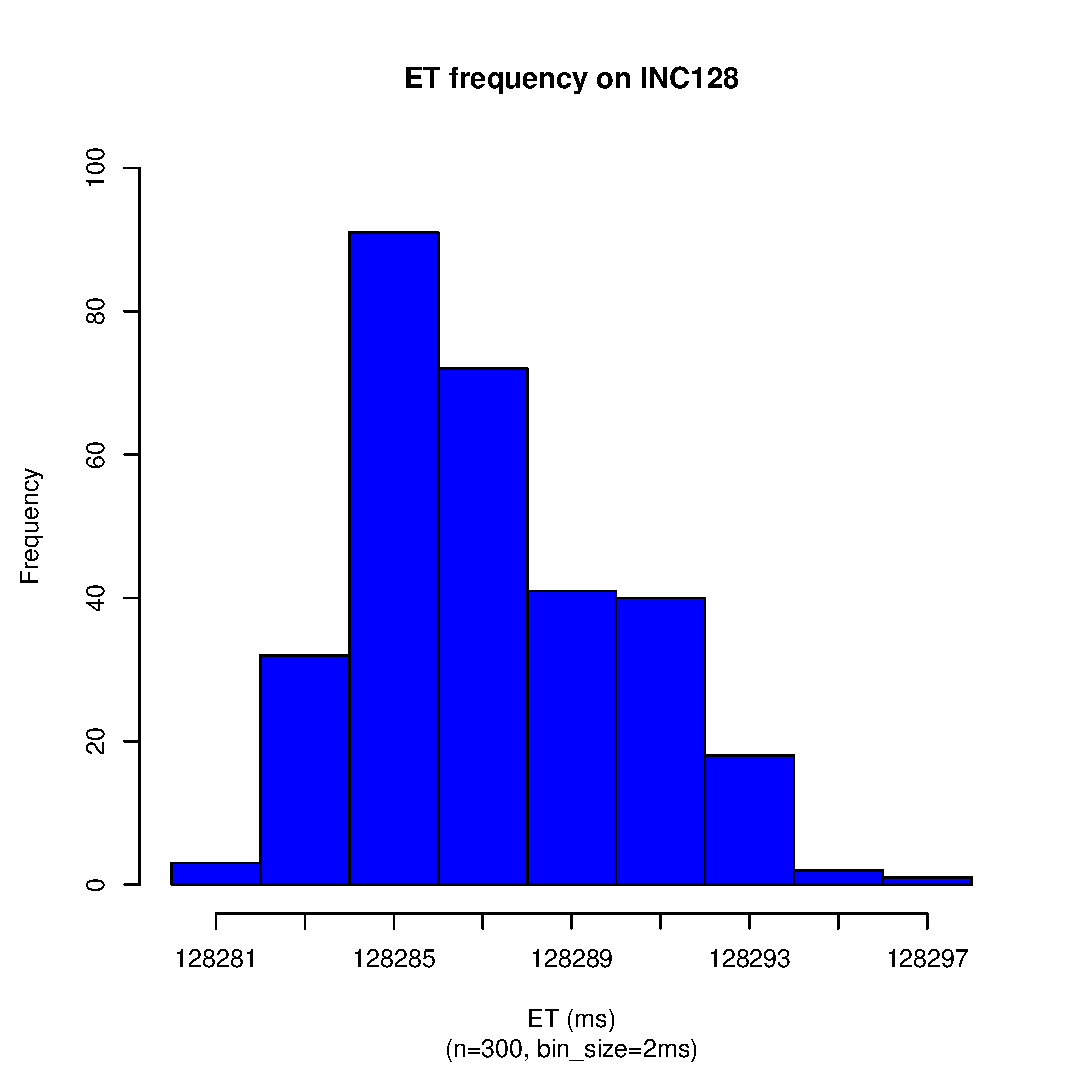
\includegraphics[scale=0.43]{repet_data2/128_sec_et_hist_v5.eps}
		\label{fig:inc128_r2_et_hist_v5}
	}
	\subfigure[ET frequency on INC256]{
		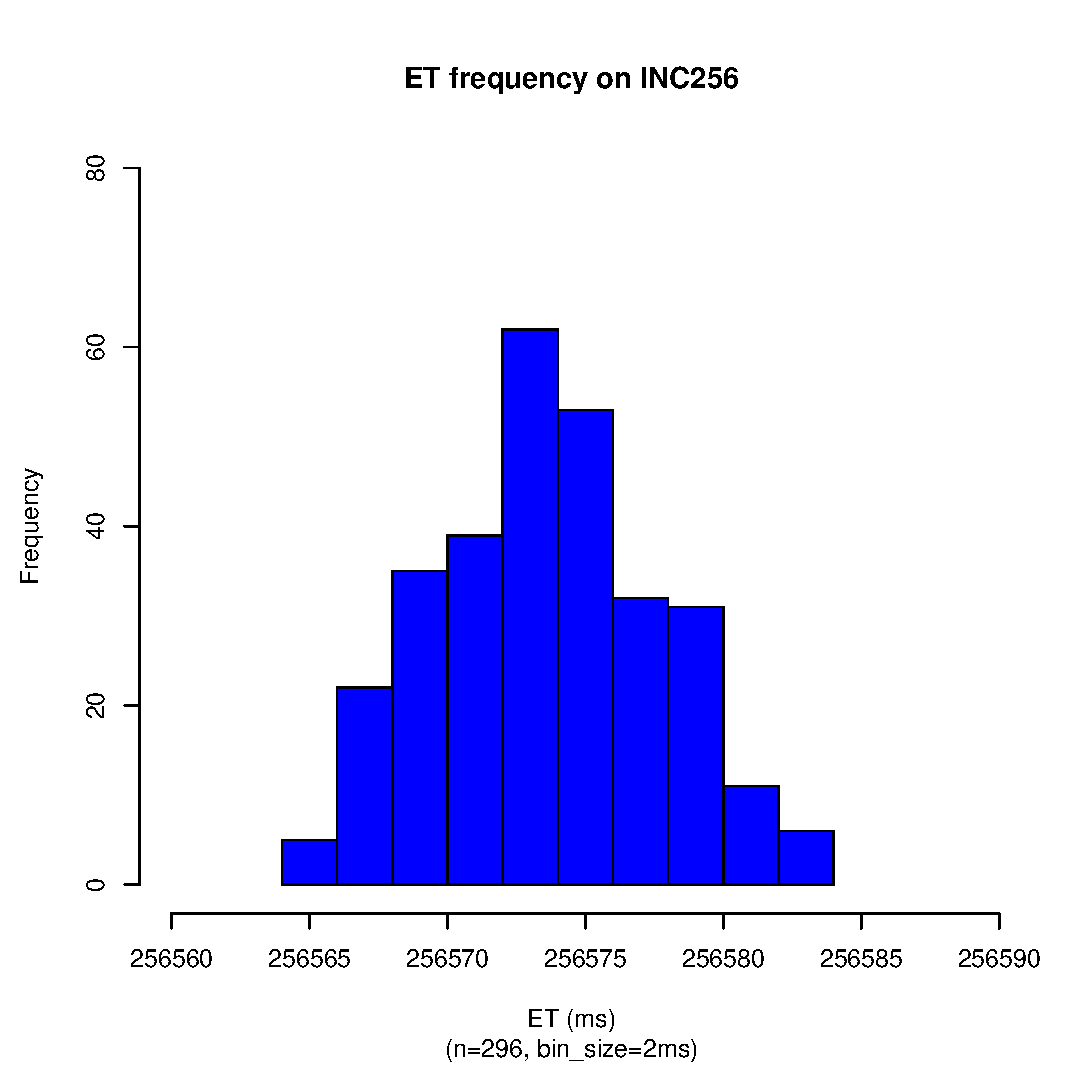
\includegraphics[scale=0.43]{repet_data2/256_sec_et_hist_v5.eps}
		\label{fig:inc256_r2_et_hist_v5}
	}
	\subfigure[ET frequency on INC512]{
		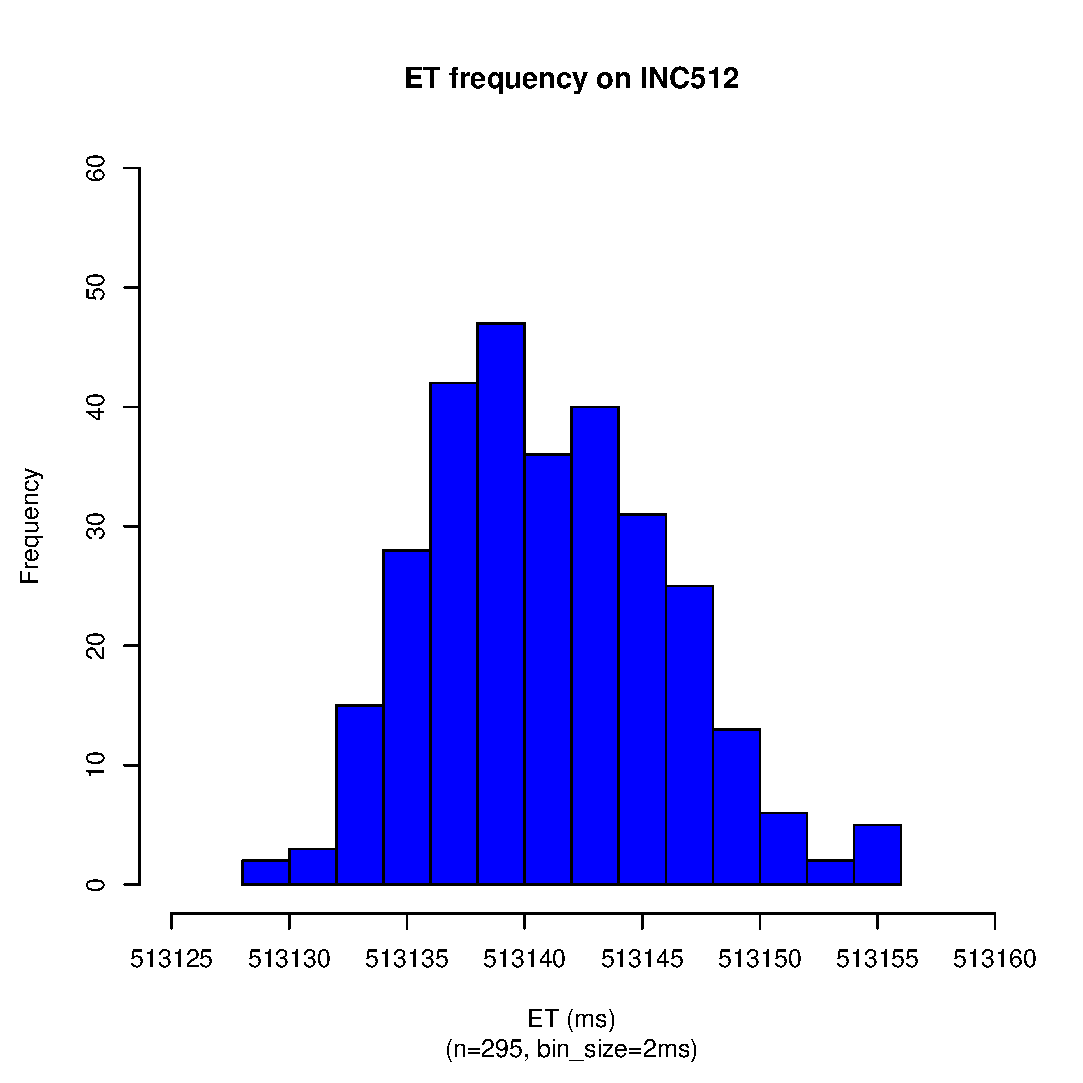
\includegraphics[scale=0.43]{repet_data2/512_sec_et_hist_v5.eps}
		\label{fig:inc512_r2_et_hist_v5}
	}
	\subfigure[ET frequency on INC1024]{
		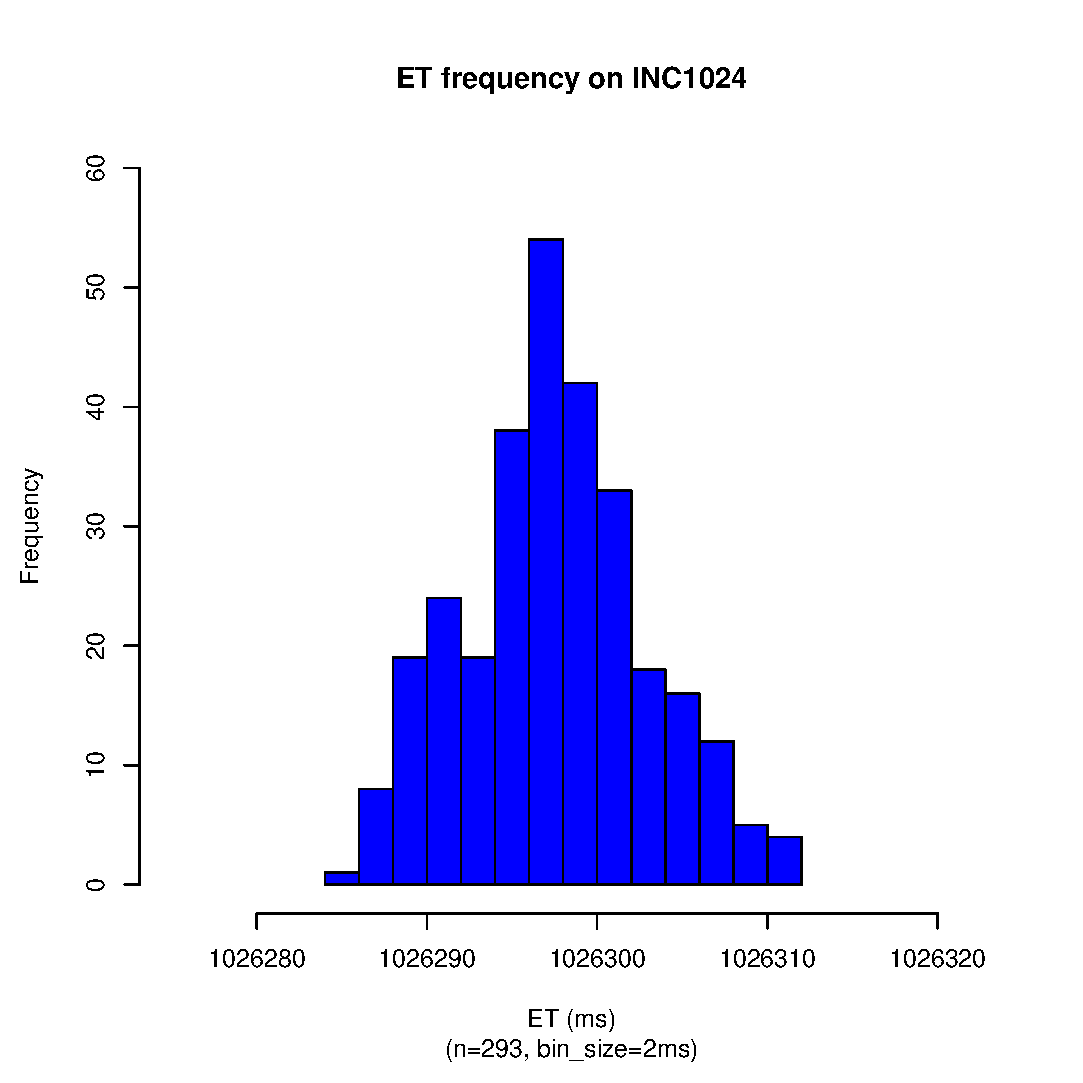
\includegraphics[scale=0.43]{repet_data2/1024_sec_et_hist_v5.eps}
		\label{fig:inc1024_r2_et_hist_v5}
	}
	\caption{ET Histograms of INC128 ... INC1024~\label{fig:s9_r2_et_hist3}}
\end{figure}

\begin{figure}[hp!]
	\centering
	\subfigure[ET frequency on INC2048]{
		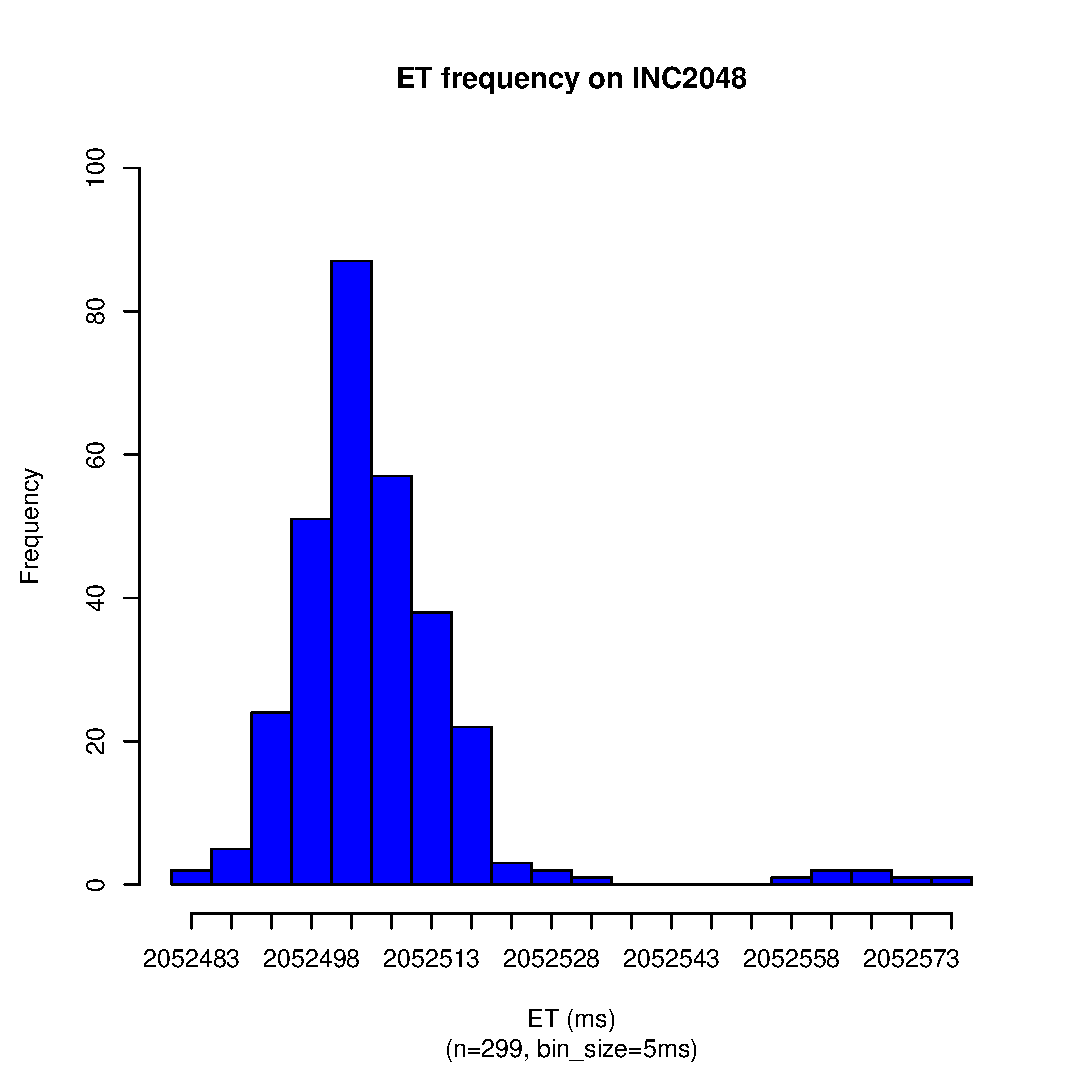
\includegraphics[scale=0.43]{repet_data2/2048_sec_et_hist_v5.eps}
		\label{fig:inc2048_r2_et_hist_v5}
	}
	\subfigure[ET frequency on INC4096]{
		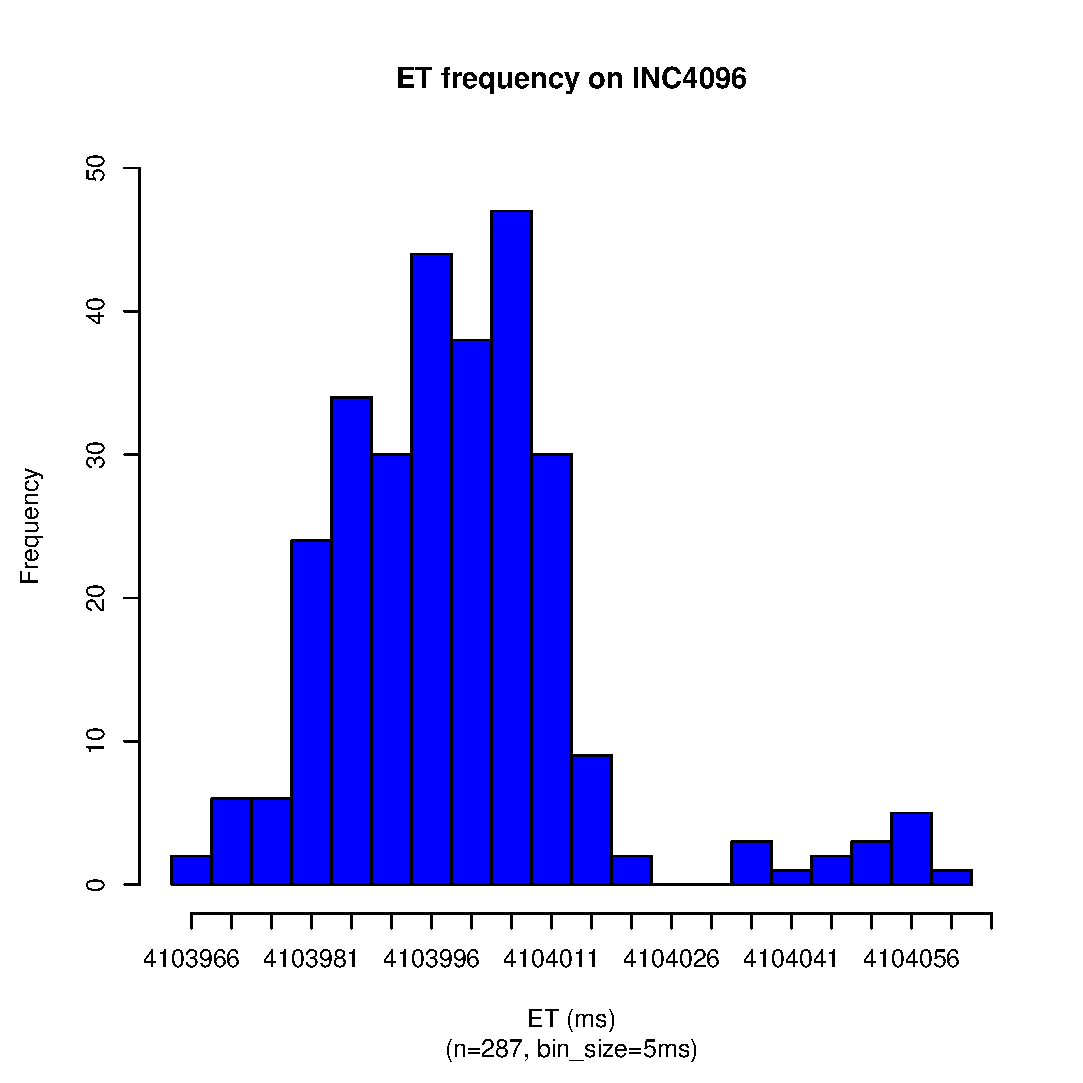
\includegraphics[scale=0.43]{repet_data2/4096_sec_et_hist_v5.eps}
		\label{fig:inc4096_r2_et_hist_v5}
	}
	\caption{ET Histograms of INC2048 and INC4096~\label{fig:s9_r2_et_hist4}}
\end{figure}

\vspace\fill
\clearpage

\subsection{PT}

\begin{figure}[hp!]
	\centering
	\subfigure[PT frequency on INC1]{
		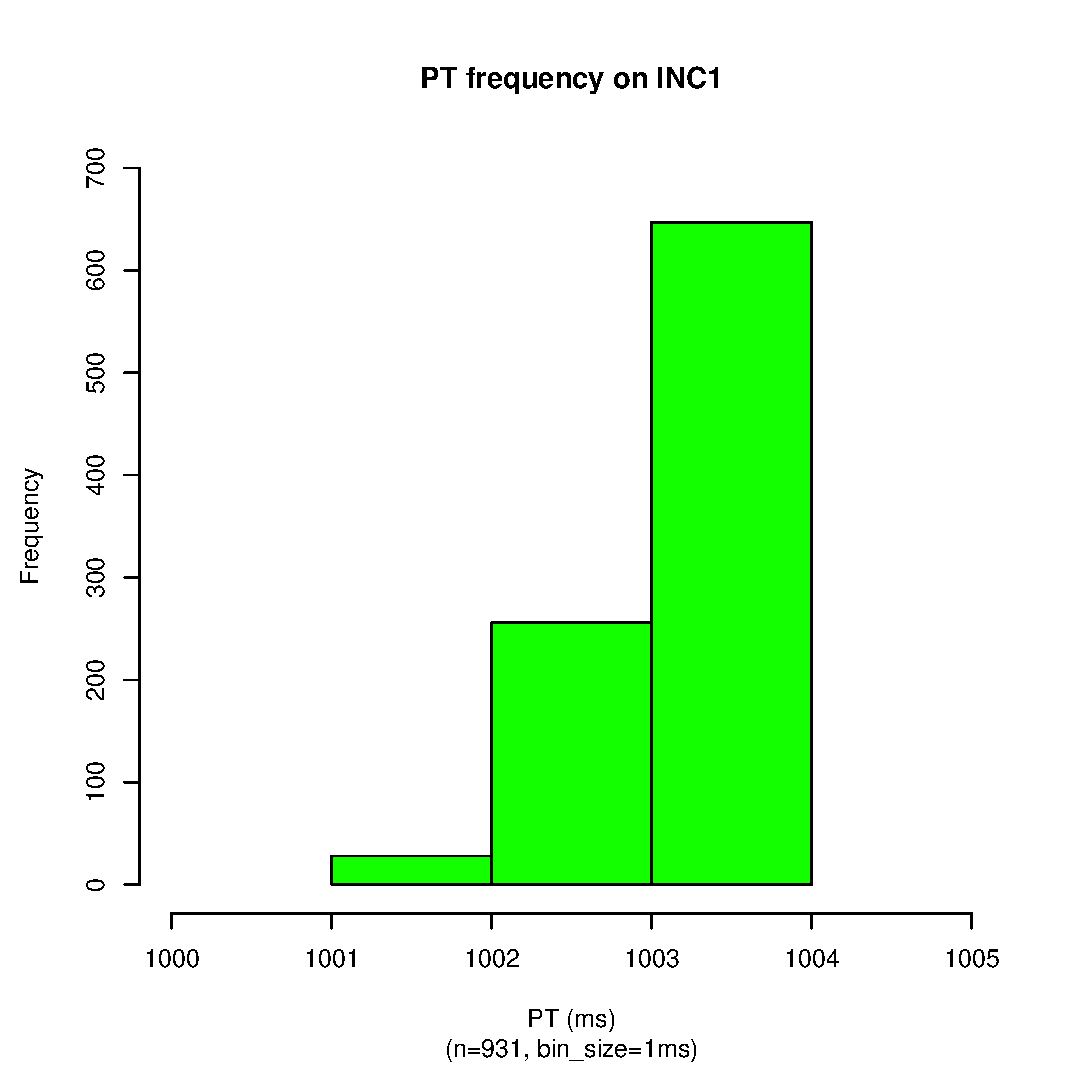
\includegraphics[scale=0.43]{repet_data2/1_sec_pt_hist_v5.eps}
		\label{fig:inc1_r2_hist_v5}
	}
	\subfigure[PT frequency on INC2]{
		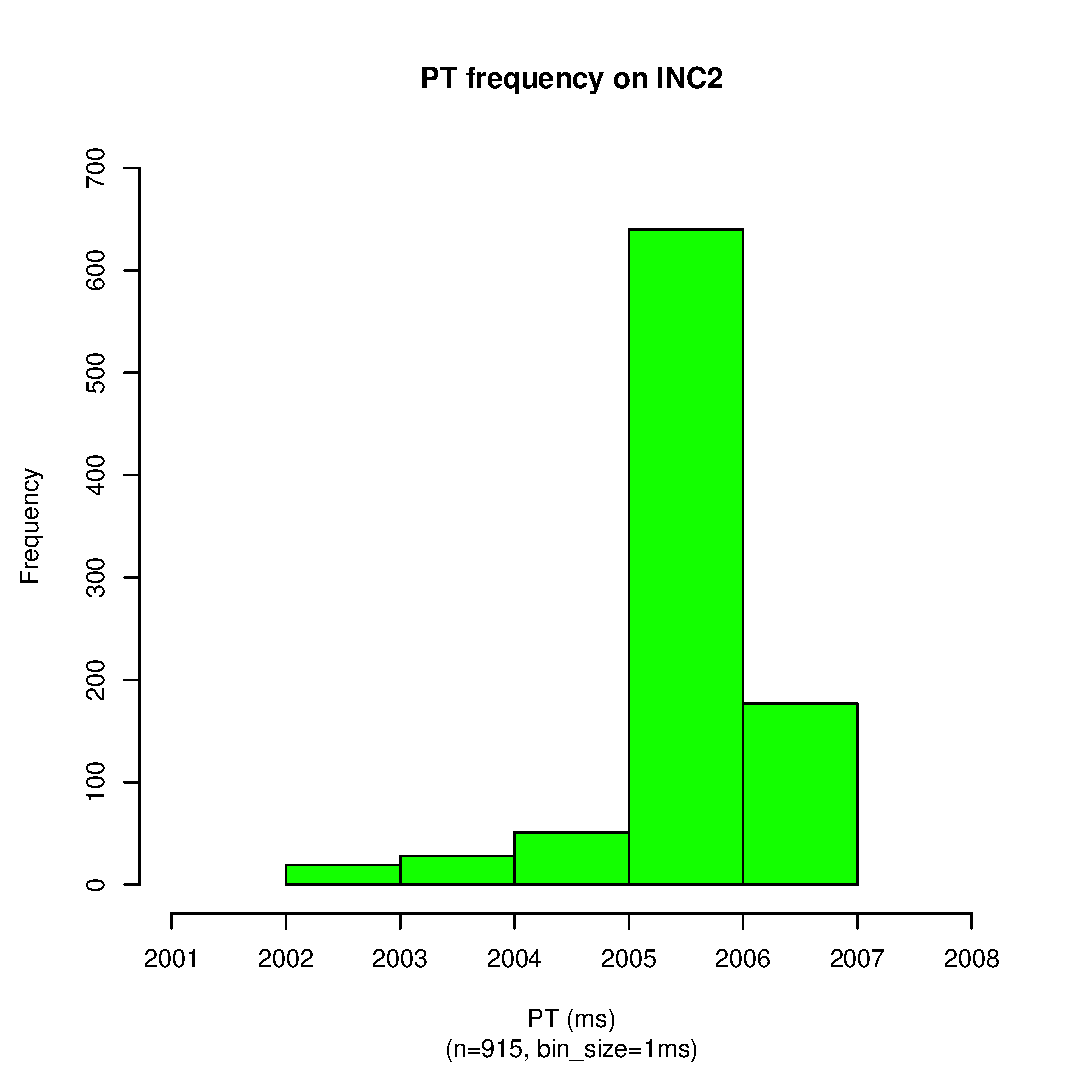
\includegraphics[scale=0.43]{repet_data2/2_sec_pt_hist_v5.eps}
		\label{fig:inc2_r2_hist_v5}
	}
	\subfigure[PT frequency on INC4]{
		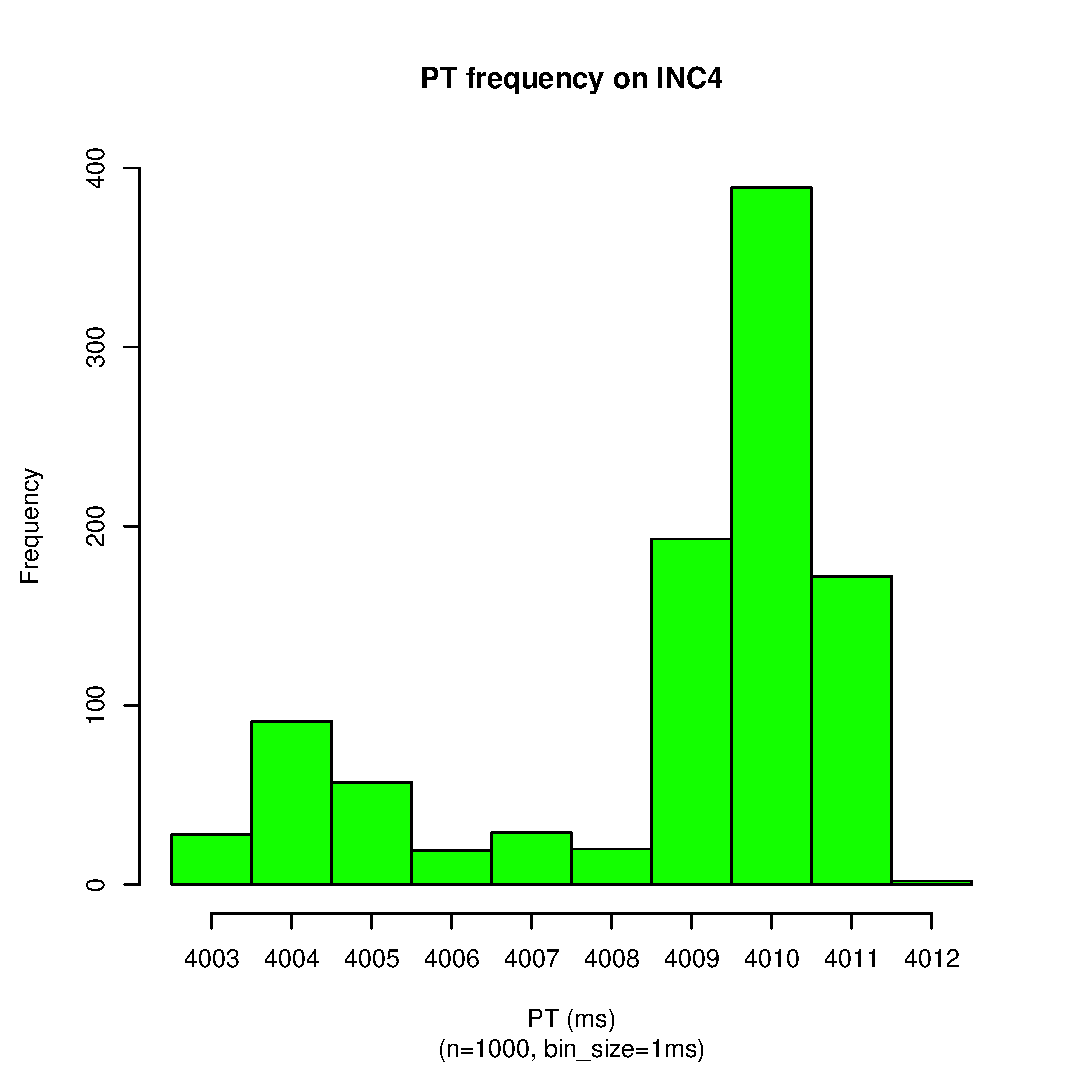
\includegraphics[scale=0.43]{repet_data2/4_sec_pt_hist_v5.eps}
		\label{fig:inc4_r2_hist_v5}
	}
	\subfigure[PT frequency on INC8]{
		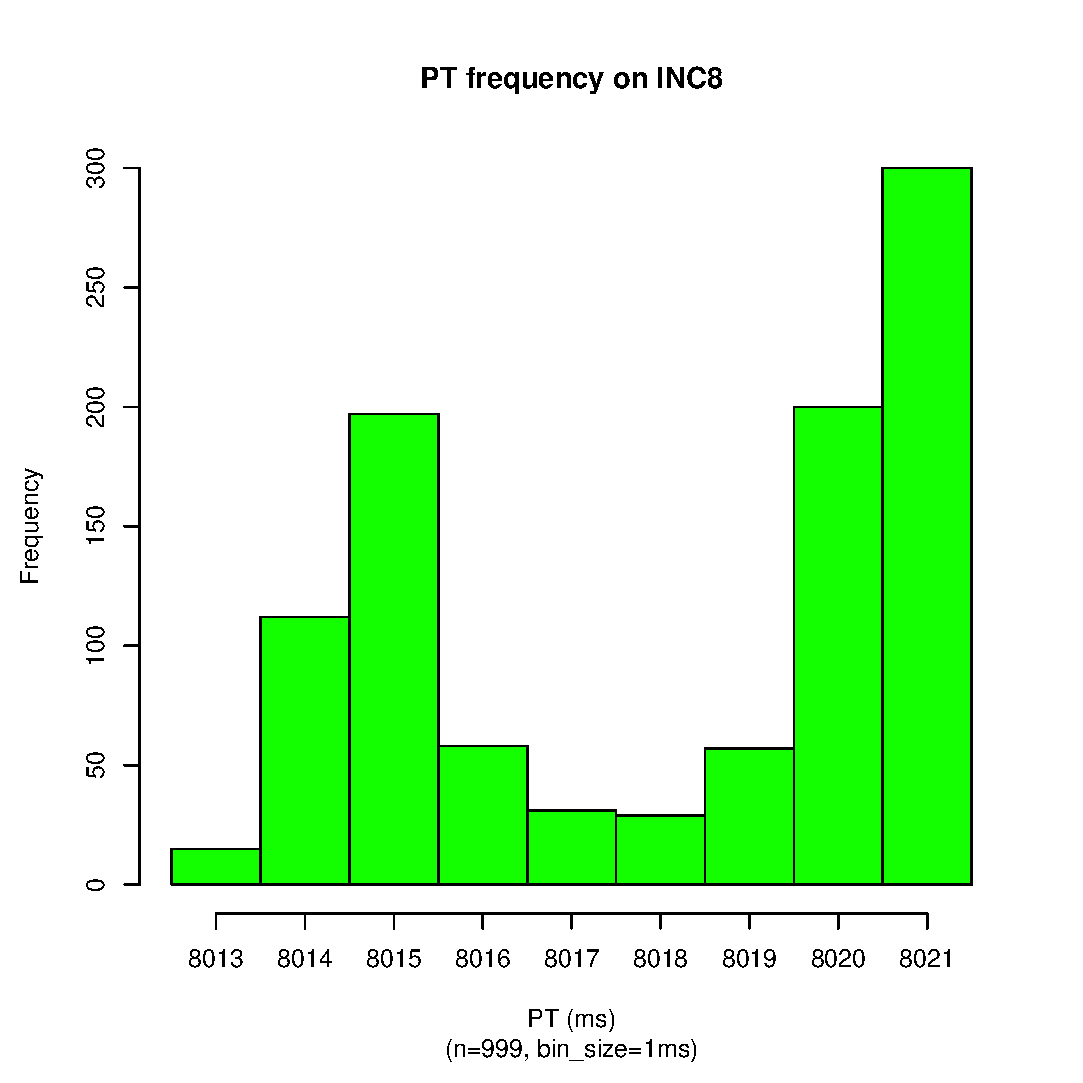
\includegraphics[scale=0.43]{repet_data2/8_sec_pt_hist_v5.eps}
		\label{fig:inc8_r2_hist_v5}
	}
	\caption{PT Histograms of INC1 ... INC8~\label{fig:s9_r2_pt_hist1}}
\end{figure}

\begin{figure}[hp!]
	\centering
	\subfigure[PT frequency on INC16]{
		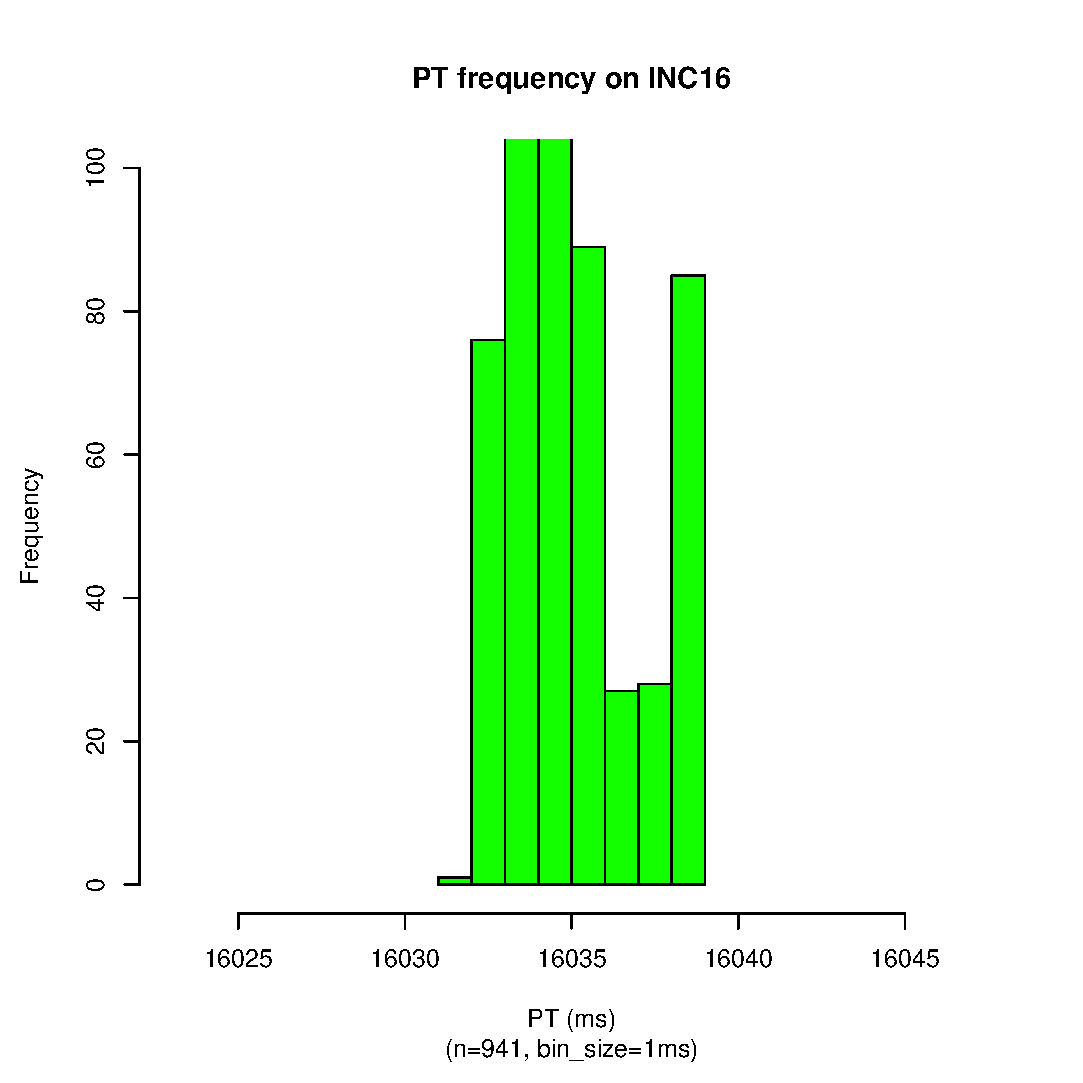
\includegraphics[scale=0.43]{repet_data2/16_sec_pt_hist_v5.eps}
		\label{fig:inc16_r2_hist_v5}
	}
	\subfigure[PT frequency on INC32]{
		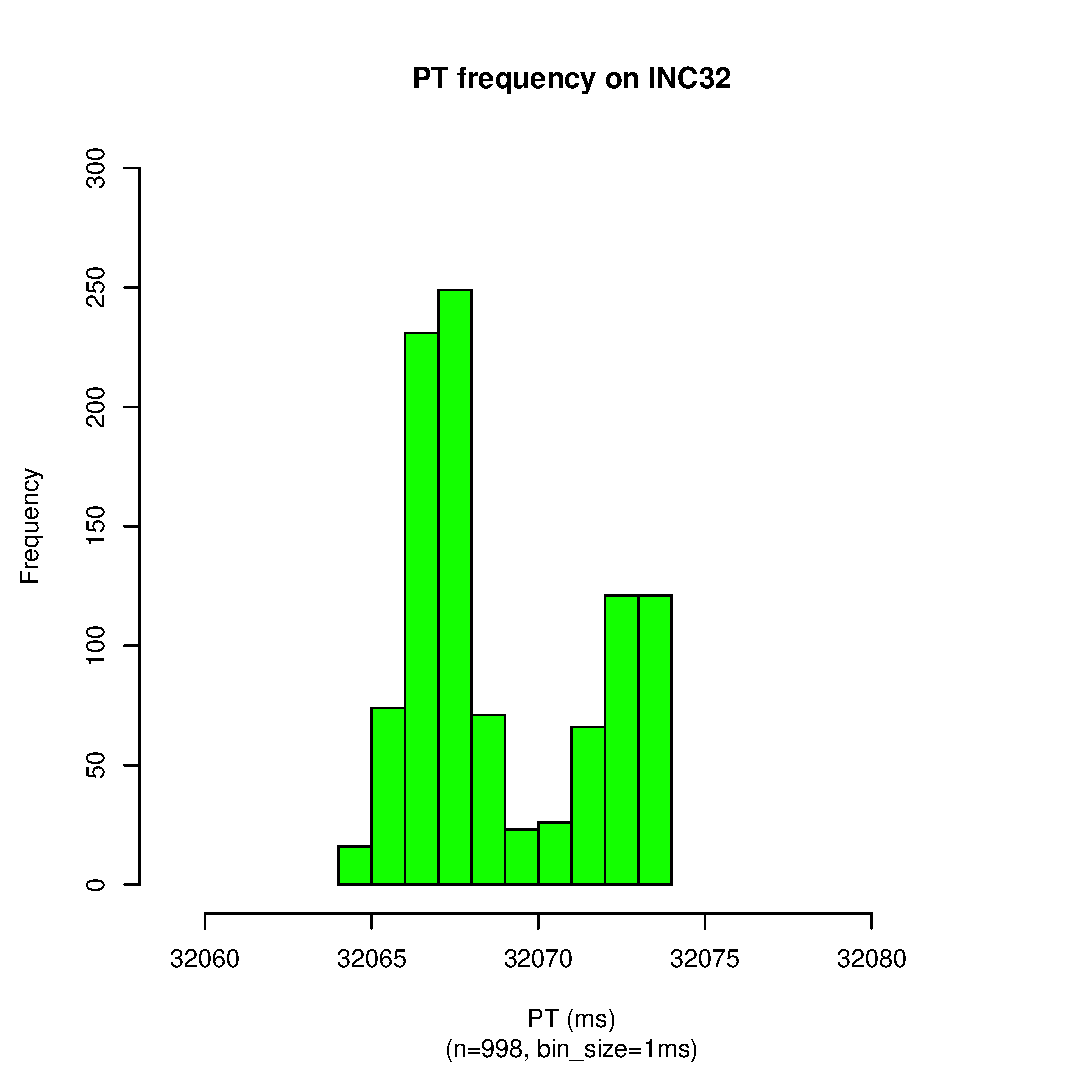
\includegraphics[scale=0.43]{repet_data2/32_sec_pt_hist_v5.eps}
		\label{fig:inc32_r2_hist_v5}
	}
	\subfigure[PT frequency on INC64]{
		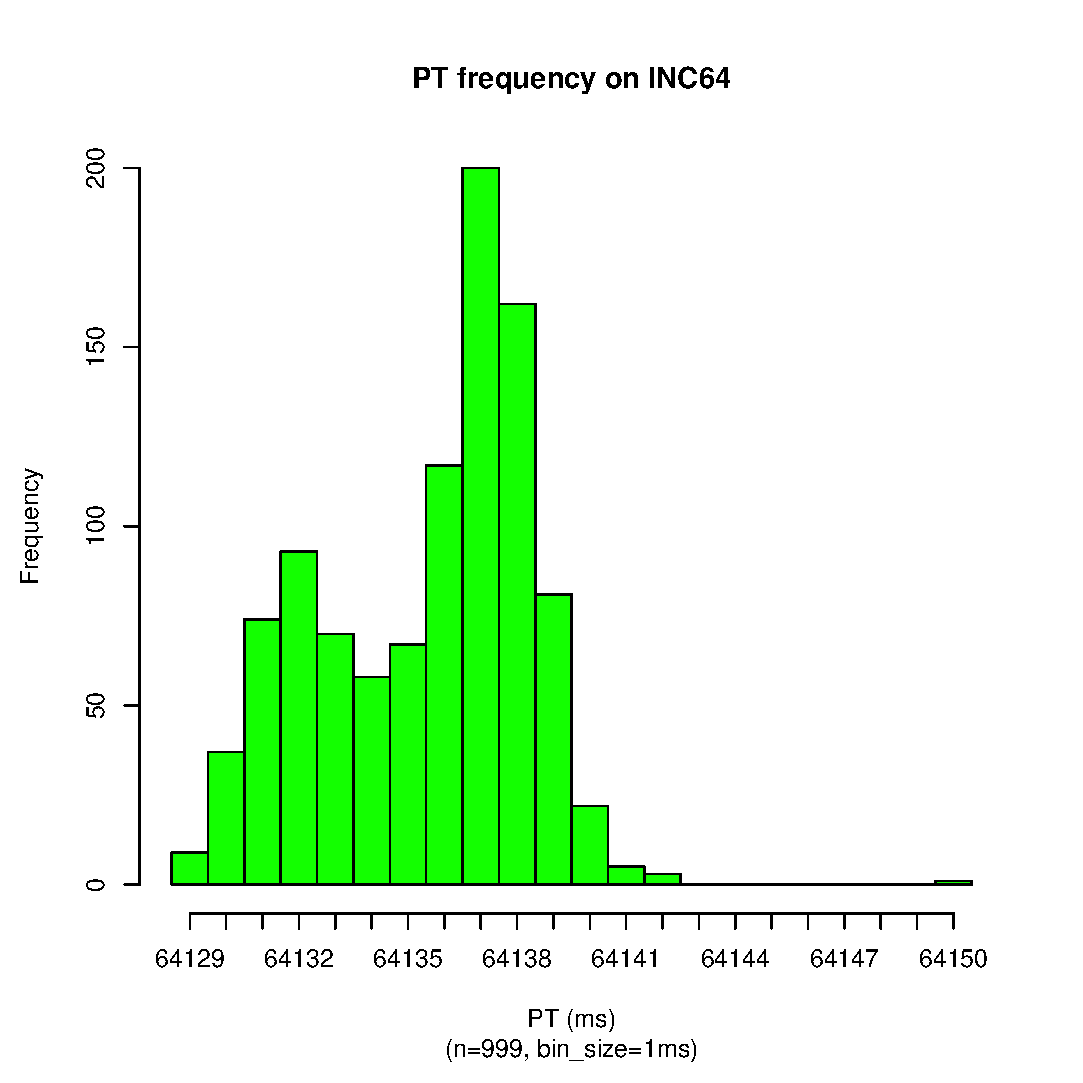
\includegraphics[scale=0.43]{repet_data2/64_sec_pt_hist_v5.eps}
		\label{fig:inc64_r2_hist_v5}
	}
	\caption{PT Histograms of INC16 ... INC64\label{fig:s9_r2_pt_hist2}}
\end{figure}

\begin{figure}[hp!]
	\centering
	\subfigure[PT frequency on INC128]{
		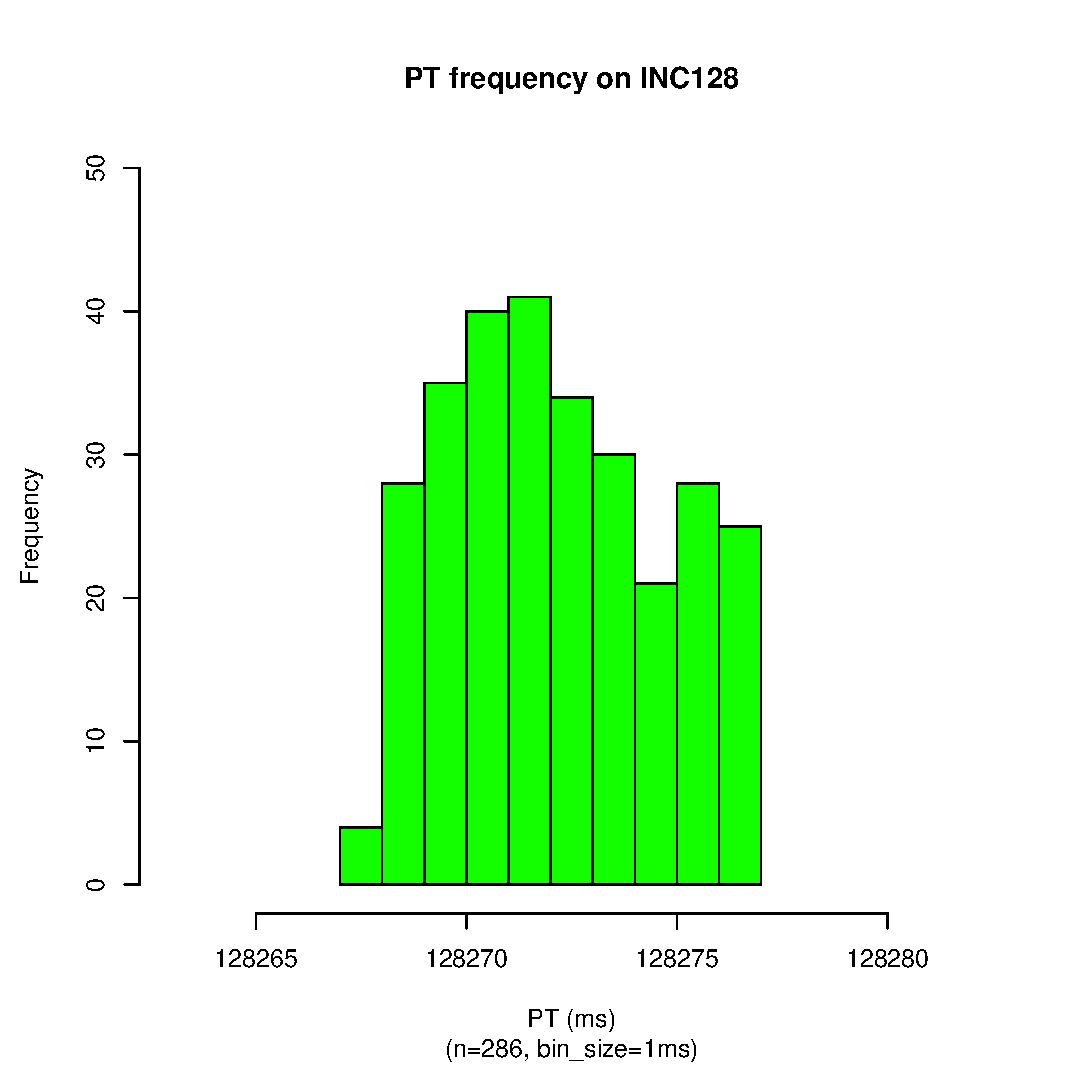
\includegraphics[scale=0.43]{repet_data2/128_sec_pt_hist_v5.eps}
		\label{fig:inc128_r2_hist_v5}
	}
	\subfigure[PT frequency on INC256]{
		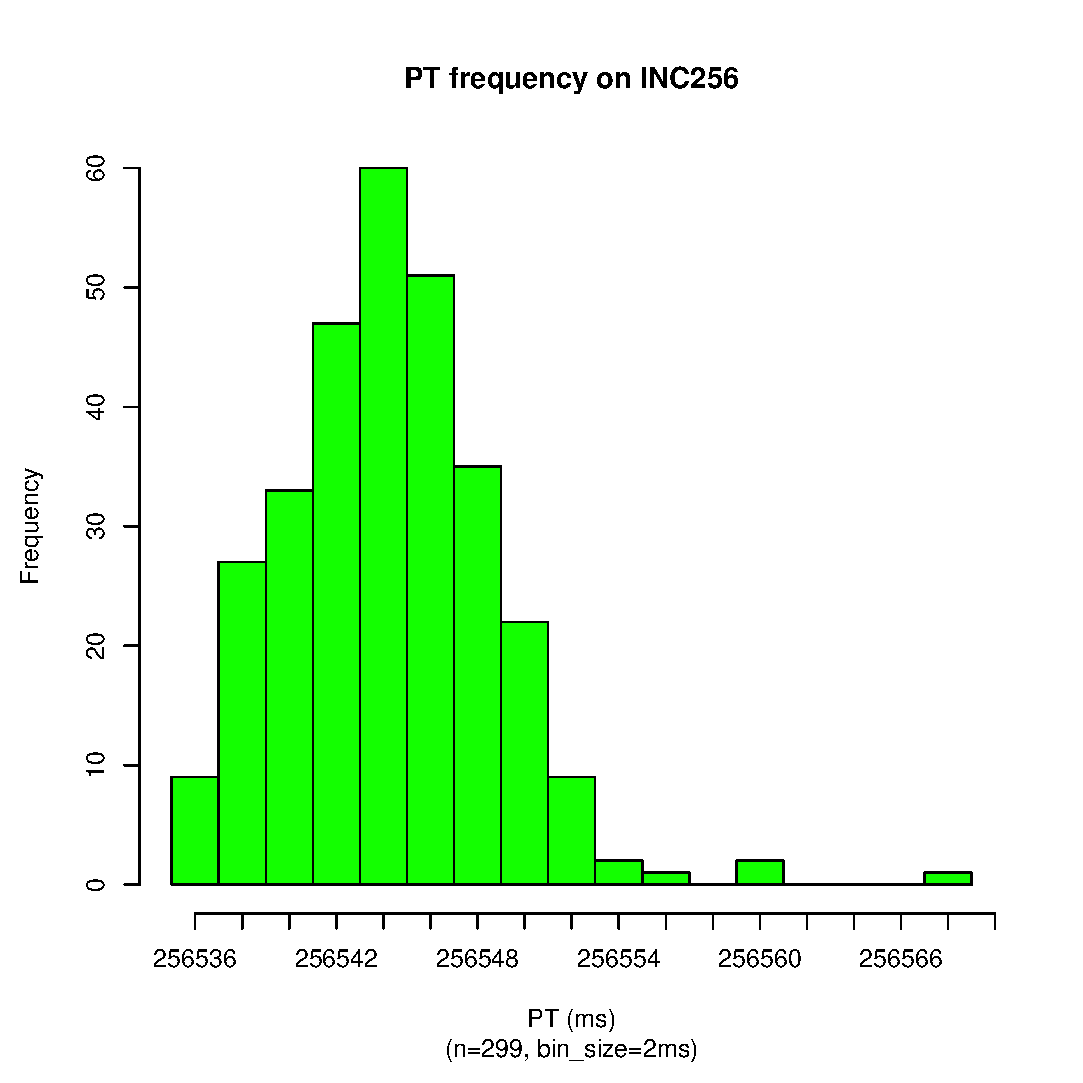
\includegraphics[scale=0.43]{repet_data2/256_sec_pt_hist_v5.eps}
		\label{fig:inc256_r2_hist_v5}
	}
	\subfigure[PT frequency on INC512]{
		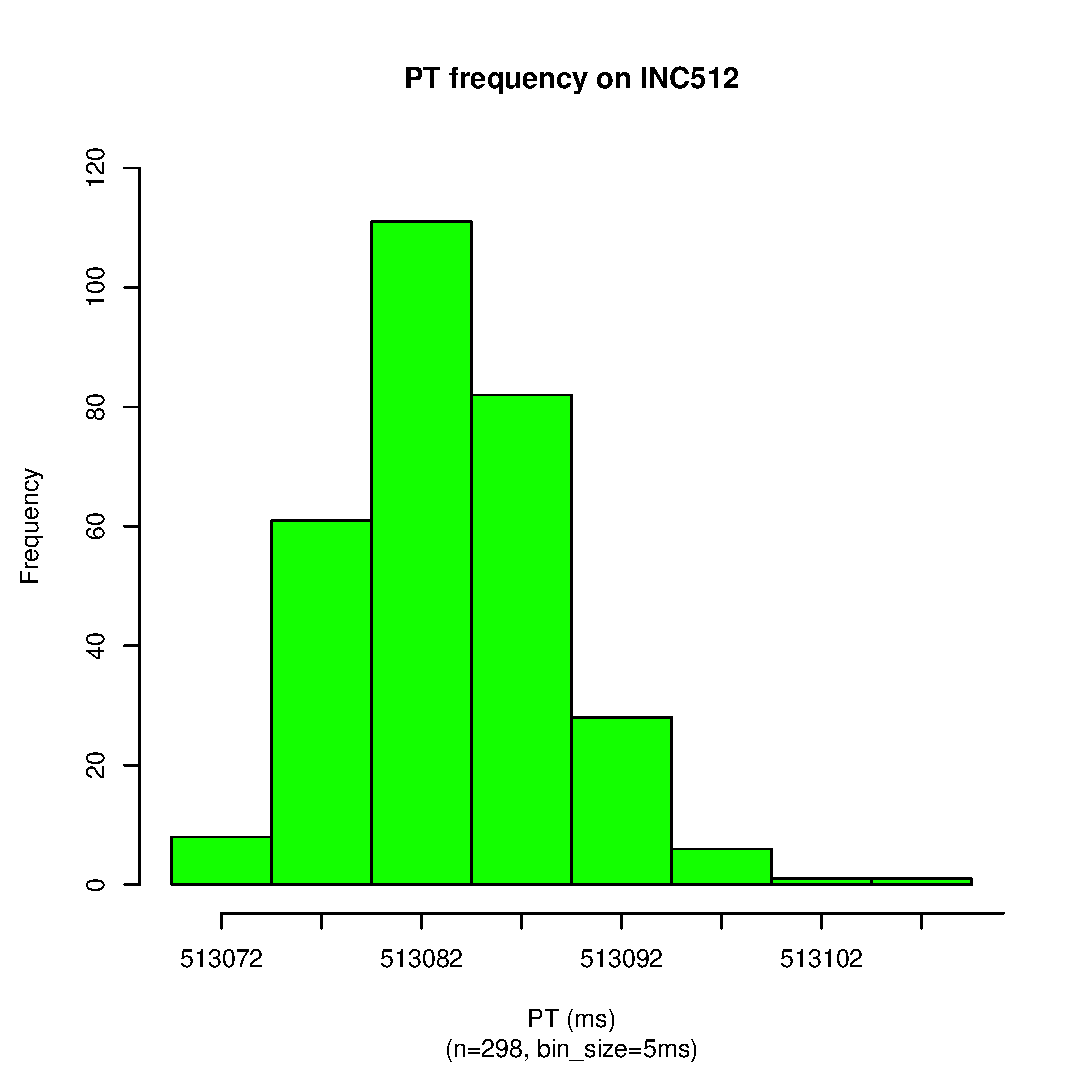
\includegraphics[scale=0.43]{repet_data2/512_sec_pt_hist_v5.eps}
		\label{fig:inc512_r2_hist_v5}
	}
	\subfigure[PT frequency on INC1024]{
		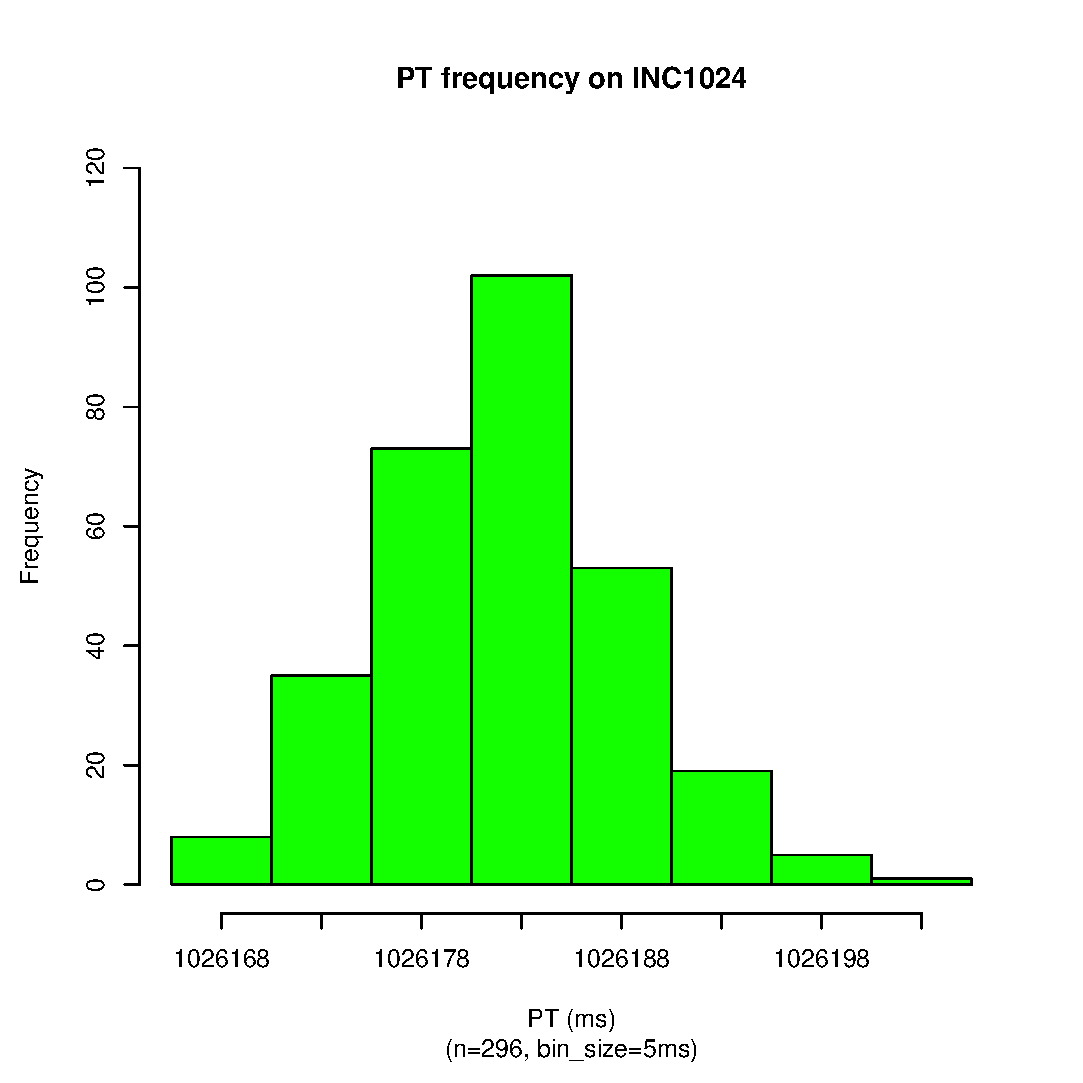
\includegraphics[scale=0.43]{repet_data2/1024_sec_pt_hist_v5.eps}
		\label{fig:inc1024_r2_hist_v5}
	}
	\caption{PT Histograms of INC256 ... INC1024~\label{fig:s9_r2_pt_hist3}}
\end{figure}

\begin{figure}[t]
	\centering
	\subfigure[PT frequency on INC2048]{
		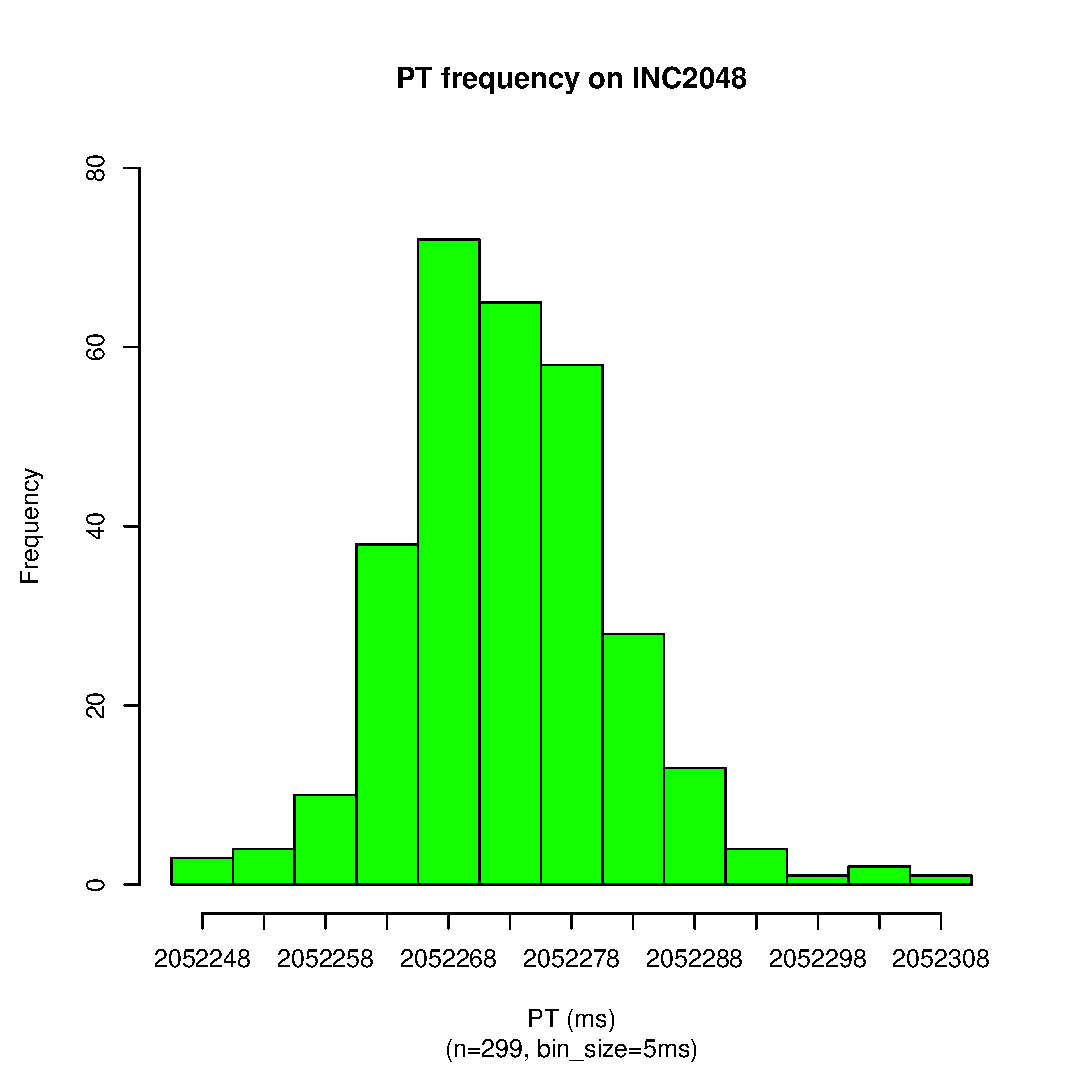
\includegraphics[scale=0.43]{repet_data2/2048_sec_pt_hist_v5.eps}
		\label{fig:inc2048_r2_hist_v5}
	}
	\subfigure[PT frequency on INC4096]{
		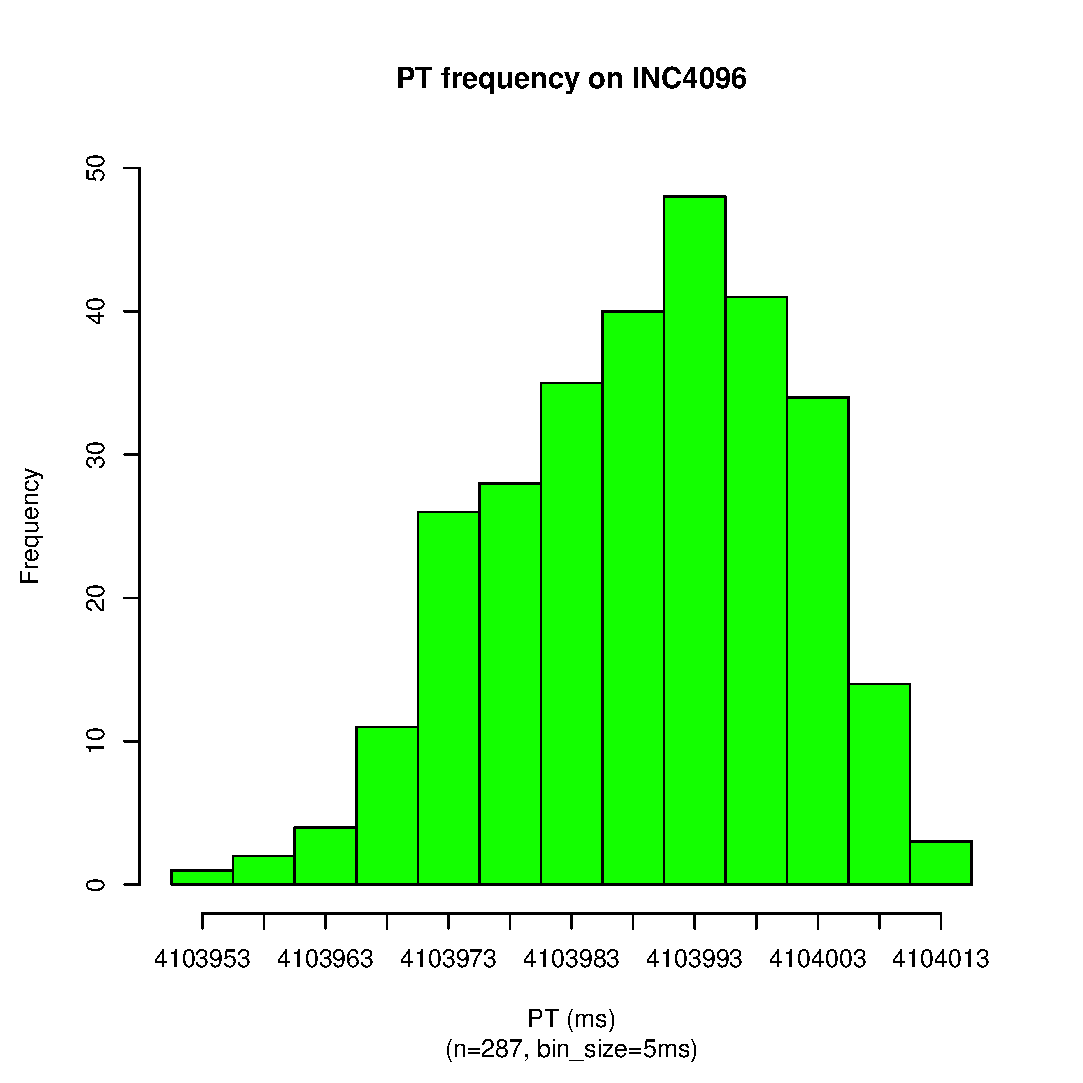
\includegraphics[scale=0.43]{repet_data2/4096_sec_pt_hist_v5.eps}
		\label{fig:inc4096_r2_hist_v5}
	}
	\caption{PT Histograms of INC2048 and INC4096~\label{fig:s9_r2_pt_hist4}}
\end{figure}

\clearpage
\pagebreak
\subsubsection{Analysis}
In this section we look into what happened inside the peaks observed in a certain histogram. 
We consider Figure~\ref{fig:inc8_r2_hist_v5} for this study. 
In the figure, we see the peaks at 8015 msec, 8020 msec, and 8021 msec. 

Table~\ref{tab:inc8_daemons} shows captured daemons and their runtime statistics per bin 
of figure. Note that bin is at the unit of PT. 
It appears that the peaks are definitely correlated with (1) appearances of some daemons 
and (2) times that those daemons co-ran with INC8. 

\begin{table}[h]
\begin{center}
{\scriptsize
\begin{tabular}{l|l|l|l|l|l|l|l} \hline
TASK\_LEN  & BIN (PT) &  DAEMON   & MIN\_PT  &  MAX\_PT  &  AVG\_PT  &   STD\_PT & Counts \\ \hline
INC8     & 8013  & jbd2/md0-8    & 1     & 1     & 1     & 0     & 1\\ \hline
INC8     & 8013  & kslowd000     & 1     & 1     & 1     & 0     & 1\\ \hline
INC8     & 8013  & md0\_raid1     & 1     & 1     & 1     & 0     & 17\\ \hline
INC8     & 8013  & proc\_monitor  & 196   & 200   & 197.72        & 1.07  & 18\\ \hline \hline

INC8     & 8014  & jbd2/md0-8    & 1     & 1     & 1     & 0     & 5\\ \hline
INC8     & 8014  & kslowd000     & 1     & 1     & 1     & 0     & 35\\ \hline
INC8     & 8014  & kslowd001     & 1     & 1     & 1     & 0     & 26\\ \hline
INC8     & 8014  & md0\_raid1     & 1     & 1     & 1     & 0     & 58\\ \hline
INC8     & 8014  & proc\_monitor  & 196   & 200   & 197.31        & 1.06  & 95\\ \hline \hline

INC8     & {\bf 8015}  & java  & 2     & 7     & 4.5   & 3.54  & 2\\ \hline
INC8     & {\bf 8015}  & jbd2/md0-8    & 1     & 1     & 1     & 0     & 2\\ \hline
INC8     & {\bf 8015}  & kslowd000     & 1     & 1     & 1     & 0     & 86\\ \hline
INC8     & {\bf 8015}  & kslowd001     & 1     & 1     & 1     & 0     & 89\\ \hline
INC8     & {\bf 8015}  & md0\_raid1     & 1     & 1     & 1     & 0     & 18\\ \hline
INC8     & {\bf 8015}  & proc\_monitor  & 196   & 200   & 197.28        & 1.01  & 194\\ \hline\hline

INC8     & 8016  & kslowd000     & 1     & 1     & 1     & 0     & 36\\ \hline
INC8     & 8016  & kslowd001     & 1     & 1     & 1     & 0     & 40\\ \hline
INC8     & 8016  & md0\_raid1     & 1     & 1     & 1     & 0     & 8\\ \hline
INC8     & 8016  & proc\_monitor  & 196   & 200   & 196.45        & .95   & 78\\ \hline\hline

INC8     & 8017  & kslowd000     & 1     & 1     & 1     & 0     & 11\\ \hline
INC8     & 8017  & kslowd001     & 1     & 1     & 1     & 0     & 10\\ \hline
INC8     & 8017  & md0\_raid1     & 1     & 1     & 1     & 0     & 3\\ \hline
INC8     & 8017  & proc\_monitor  & 196   & 200   & 197.15        & 1.16  & 26\\ \hline\hline

INC8     & 8018  & kslowd000     & 1     & 1     & 1     & 0     & 13\\ \hline
INC8     & 8018  & kslowd001     & 1     & 1     & 1     & 0     & 9\\ \hline
INC8     & 8018  & md0\_raid1     & 1     & 1     & 1     & 0     & 6\\ \hline
INC8     & 8018  & proc\_monitor  & 196   & 200   & 197.24        & 1.27  & 29\\ \hline\hline

INC8     & 8019  & jbd2/md0-8    & 1     & 1     & 1     & 0     & 3\\ \hline
INC8     & 8019  & kslowd000     & 1     & 1     & 1     & 0     & 9\\ \hline
INC8     & 8019  & kslowd001     & 1     & 2     & 1.06  & .24   & 18\\ \hline
INC8     & 8019  & md0\_raid1     & 1     & 1     & 1     & 0     & 27\\ \hline
INC8     & 8019  & proc\_monitor  & 196   & 200   & 197.1         & 1.18  & 52\\ \hline\hline

INC8     & {\bf 8020}  & jbd2/md0-8    & 1     & 1     & 1     & 0     & 8\\ \hline
INC8     & {\bf 8020}  & kslowd000     & 1     & 1     & 1     & 0     & 52\\ \hline
INC8     & {\bf 8020}  & kslowd001     & 1     & 1     & 1     & 0     & 57\\ \hline
INC8     & {\bf 8020}  & md0\_raid1     & 1     & 1     & 1     & 0     & 91\\ \hline
INC8     & {\bf 8020}  & proc\_monitor  & 196   & 200   & 197.03        & 1.02  & 180\\ \hline\hline

INC8     & {\bf 8021}  & cifsd         & 1     & 1     & 1     & 0     & 1\\ \hline
INC8     & {\bf 8021}  & java  & 2     & 37    & 19.5  & 24.75         & 2\\ \hline
INC8     & {\bf 8021}  & kslowd000     & 1     & 1     & 1     & 0     & 146\\ \hline
INC8     & {\bf 8021}  & kslowd001     & 1     & 1     & 1     & 0     & 143\\ \hline
INC8     & {\bf 8021}  & md0\_raid1     & 1     & 1     & 1     & 0     & 11\\ \hline
INC8     & {\bf 8021}  & proc\_monitor  & 196   & 198   & 197.15        & .98   & 299\\ \hline\hline

INC8     & 8022  & kslowd000     & 1     & 1     & 1     & 0     & 20\\ \hline
INC8     & 8022  & kslowd001     & 1     & 1     & 1     & 0     & 9\\ \hline
INC8     & 8022  & proc\_monitor  & 196   & 198   & 196.07        & .37   & 29\\ \hline\hline
\end{tabular}
}
\end{center}
\caption{Daemons observed from the INC8 run~\label{tab:inc8_daemons}}
\end{table}

